\documentclass[paper=a4, fontsize=10pt]{scrartcl} % A4 paper and 11pt font size

\usepackage[T1]{fontenc} % Use 8-bit encoding that has 256 glyphs
\usepackage{fourier} % Use the Adobe Utopia font for the document - comment this line to return to the LaTeX default
\usepackage[english]{babel} % English language/hyphenation
\usepackage{amsmath,amsfonts,amsthm} % Math packages
\usepackage{graphicx}
\usepackage[cm]{fullpage}
\usepackage{float}
\usepackage{sectsty} % Allows customizing section commands
\allsectionsfont{\centering \normalfont\scshape} % Make all sections centered, the default font and small caps

\usepackage{fancyhdr} % Custom headers and footers
\pagestyle{fancyplain} % Makes all pages in the document conform to the custom headers and footers
\fancyhead{} % No page header - if you want one, create it in the same way as the footers below
\fancyfoot[L]{} % Empty left footer
\fancyfoot[C]{} % Empty center footer
\fancyfoot[R]{\thepage} % Page numbering for right footer
\renewcommand{\headrulewidth}{0pt} % Remove header underlines
\renewcommand{\footrulewidth}{0pt} % Remove footer underlines
\setlength{\headheight}{13.6pt} % Customize the height of the header

\numberwithin{equation}{section} % Number equations within sections (i.e. 1.1, 1.2, 2.1, 2.2 instead of 1, 2, 3, 4)
\numberwithin{figure}{section} % Number figures within sections (i.e. 1.1, 1.2, 2.1, 2.2 instead of 1, 2, 3, 4)
\numberwithin{table}{section} % Number tables within sections (i.e. 1.1, 1.2, 2.1, 2.2 instead of 1, 2, 3, 4)

\setlength\parindent{0pt} % Removes all indentation from paragraphs - comment this line for an assignment with lots of text

%----------------------------------------------------------------------------------------
%	TITLE SECTION
%----------------------------------------------------------------------------------------

\newcommand{\horrule}[1]{\rule{\linewidth}{#1}} % Create horizontal rule command with 1 argument of height

\title{	
\normalfont \normalsize 
\textsc{Radboud University Nijmegen}  % Your university, school and/or department name(s)
\horrule{0.5pt} \\[0.3cm] % Thin top horizontal rule
\huge Statistical Machine Learning \\ Assignment 1 \\ % The assignment title
\horrule{2pt}  % Thick bottom horizontal rule
}

\author{Steven Reitsma \\ (s4132343)} % Your name

\date{\normalsize\today} % Today's date or a custom date

\begin{document}

\maketitle % Print the title

\section{Polynomial Curve Fitting}
\subsection{Plotting a noisy function}
\begin{figure}[H]
	\centering
	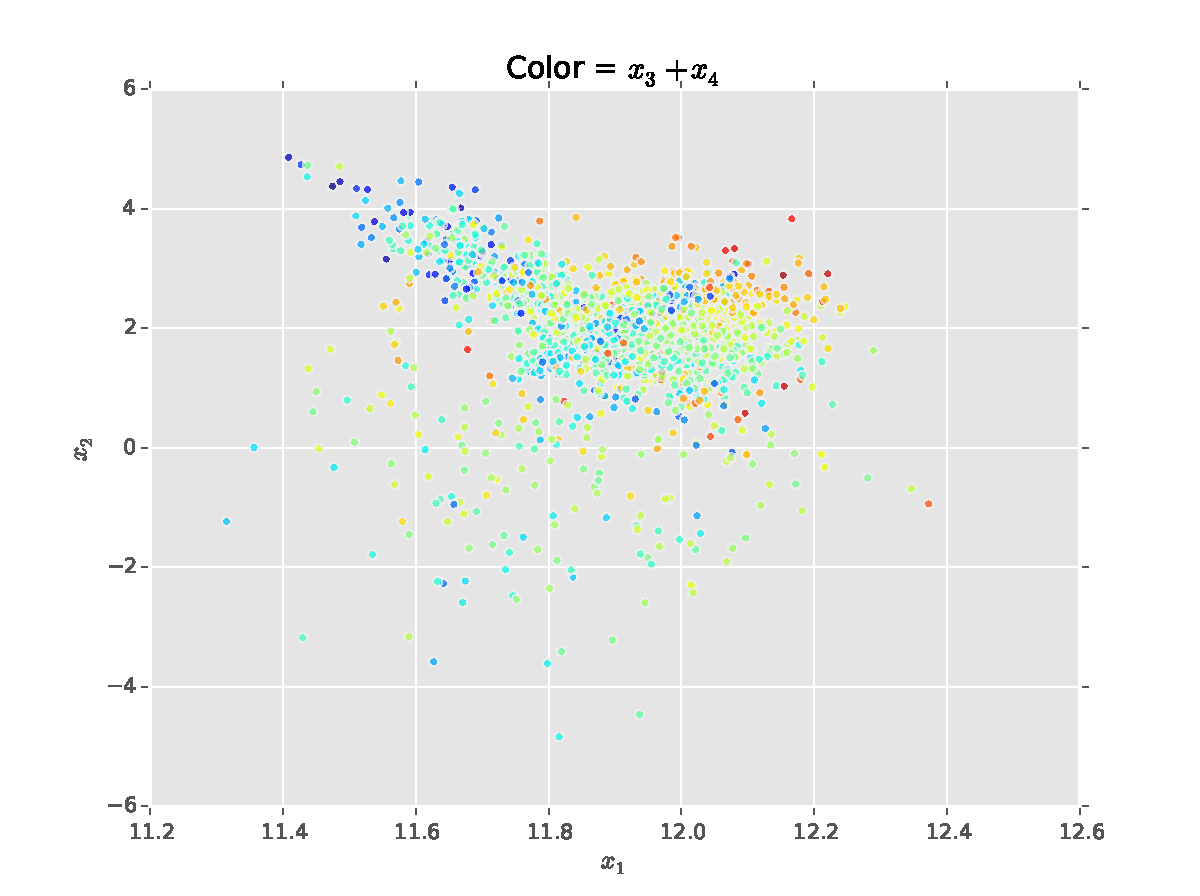
\includegraphics[width=0.9\linewidth]{exercise_11.pdf}
	\caption{The real sinusoid and 10 noisy data observations plotted.}
\end{figure}

The code for this exercise can be found in file $\verb|exercise_11.py|$.

\subsection{Fitting the polynomial}
See $\verb|exercise_12_13_14_15.py|$ for the code.

\subsection{Plotting the polynomials}
Please note that due to the random nature of the Gaussian sampling, the $D_{10}$ data set used in this section is different from the set in section 1.1.
\begin{figure}[H]
	\centering
	\includegraphics[width=0.6\linewidth]{exercise_polynomial_plot.pdf}
	\caption{Polynomials with order M = 0, 1, 3 and 9 plotted together with the real sinusoid. It can be seen that M = 0 gives a single value, M = 1 gives a linear function, M = 3 follows the sinusoid rather nicely and M = 9 overfits extremely.}
\end{figure}

\begin{figure}[H]
	\centering
	\includegraphics[width=0.6\linewidth]{exercise_rmse_plot.pdf}
	\caption{This plot shows the root mean squared error (RMSE) for various polynomial orders. Note that this plot clearly shows overfitting for higher order polynomials: the training set error decreases, while the test set error increases.}
\end{figure}

\subsection{Doing the same for a data set with 40 points}
\begin{figure}[H]
	\centering
	\includegraphics[width=0.7\linewidth]{exercise_polynomial_plot40.pdf}
	\caption{Polynomials with order M = 0, 1, 3 and 9 plotted together with the real sinusoid. The difference with figure 1.2 being that the training set now contains 40 data points instead of 10. We can see that this decreases overfitting.}
\end{figure}

\begin{figure}[H]
	\centering
	\includegraphics[width=0.7\linewidth]{exercise_rmse_plot40.pdf}
	\caption{This plot shows the root mean squared error (RMSE) for various polynomial orders. Note that this plot shows less overfitting than the plot in figure 1.3, this is due to the increased size of the data set. Higher order polynomials would result in more overfitting.}
\end{figure}

\subsection{Adding regularization}
I have modified the PolCurFit function to incorporate Tikhonov regularization.
The code can be seen in the file \\$\verb|exercise_12_13_14_15.py|$. The derivation of $\tilde{E}$ is shown below.

\begin{equation}
	\tilde{E} = \frac{1}{2}\sum_{n=1}^N \{y(x_n; \bold{w}) - t_n\}^2 + \frac{\lambda}{2}\sum_{j=0}^M w_j^2
\end{equation}
\begin{equation}
	\frac{\partial\tilde{E}}{\partial w_i} = \sum_{n=1}^N(\sum_{j=0}^M w_j x_n^{i+j} - t_n x_n^i) + \frac{\partial \frac{\lambda}{2}\sum_{j=0}^M w_j^2}{\partial w_i}
\end{equation}
\begin{equation}
	\frac{\partial\tilde{E}}{\partial w_i} = \sum_{n=1}^N(\sum_{j=0}^M w_j x_n^{i+j} - t_n x_n^i) + \frac{\lambda}{2} 2 w_i
\end{equation}
\begin{equation}
	\frac{\partial\tilde{E}}{\partial w_i} = \sum_{n=1}^N(\sum_{j=0}^M w_j x_n^{i+j} - t_n x_n^i) + \lambda w_i
\end{equation}
Rewriting this to the A-matrix and T-vector notation results in:
\begin{equation}
	\frac{\partial\tilde{E}}{\partial w_i} = \sum_{n=1}^N \sum_{j=0}^M w_j x_n^{i+j} - \sum_{n=1}^N t_n x_n^i + \lambda w_i
\end{equation}
\begin{equation}
	\frac{\partial\tilde{E}}{\partial w_i} = \sum_{j=0}^N \sum_{n=1}^N x_n^{i+j} w_j - \sum_{n=1}^N t_n x_n^i + \lambda w_i
\end{equation}
\begin{equation}
	\frac{\partial\tilde{E}}{\partial w_i} = \sum_{j=0}^M A_{ij}w_j - T_i + \lambda w_i
\end{equation}
where
\begin{equation}
	A_{ij} = \sum_{n=1}^N x_n^{i+j} \qquad
	T_i = \sum_{n=1}^N t_n x_n^i
\end{equation}
Expanding this to vector notation:
\begin{equation}
	\frac{\partial\tilde{E}}{\partial w_i} = A_i\bold{w} - T_i + \lambda w_i
\end{equation}
Expanding this to all $w_i \in \bold{w}$:
\begin{equation}
	\frac{\partial\tilde{E}}{\partial \bold{w}} = A\bold{w} - \bold{T} + \lambda \bold{w}
\end{equation}
Conveniently, this equals to
\begin{equation}
	\frac{\partial\tilde{E}}{\partial \bold{w}} = (A+\lambda I)\bold{w} - \bold{T}
\end{equation}

Thus, to apply regularization, we only have to add $\lambda I$ to the A-matrix and solve the linear equations as we did before.

\begin{figure}[H]
	\centering
	\includegraphics[width=0.7\linewidth]{exercise_lambda_rmse_plot.pdf}
	\caption{This plot shows the root mean squared error (RMSE) for various values of $\lambda$ for M = 9 on the $D_{10}$ set. It strongly resembles Bishop's figure 1.8. Regularization reduces overfitting, however, too large values for $\lambda$ have an adverse effect. The higher order weights of the polynomial are driven to zero for high values of $\lambda$.}
\end{figure}

\section{Gradient descent}
\subsection{Plotting the Rosenbrock function}
\begin{figure}[H]
	\centering
	\includegraphics[width=\linewidth]{exercise_rosenbrock.png}
	\caption{A plot showing the Rosenbrock function for $a = 1$ and $b = 100$.}
\end{figure}

Initially I thought gradient descent would be easy for this function.
There are no local minima, the function looks symmetrical so there should be multiple global minima.
However, closer inspection revealed that the function is not symmetrical at all, and that the valley has a very gentle slope in itself. This leads me to believe that gradient descent will be slow to converge.

\subsection{Finding the minimum}
We want to prove that the minimum of the Rosenbrock function is (1,1). We can prove this by computing the gradient and setting it to zero.
\begin{equation}
	\nabla h(x, y) = \{ 2(200x^3 - 200xy + x - 1), 200(y - x^2) \}
\end{equation}
Setting this to zero:
\begin{equation}
	2(200x^3 - 200xy + x - 1) = 0 \qquad 200(y - x^2) = 0
\end{equation}
Solving the second equation first:
\begin{align}
	200(y - x^2) &= 0 \\
	200y - 200x^2 &= 0 \\
	200y &= 200x^2 \\
	y &= x^2 
\end{align}
Plugging this into the first equation:
\begin{align}
	2(200x^3 - 200x^3 + x - 1) &= 0 \\
	400x^3 - 400x^3 + 2x - 2) &= 0 \\
	2x - 2 &= 0 \\
	2x &= 2 \\
	x &= 1
\end{align}
Plugging this back into the second equation:
\begin{align}
200(y - 1^2) &= 0 \\
200y - 200 &= 0 \\
y - 1 &= 0 \\
y &= 1
\end{align}

\subsection{The gradient descent iteration rule}
The rule for x and y are as follows:
\begin{align}
	x_{n+1} &= x_n - \eta \nabla h(x_n,y_n) \\
	y_{n+1} &= y_n - \eta \nabla h(x_n,y_n)
\end{align}
Expanding $h(x, y)$:
\begin{align}
	x_{n+1} &= x_n - \eta (400x_n^3 - 200x_ny_n + 2x_n - 2) \\
	y_{n+1} &= y_n - \eta (200y_n - 200x_n^2)
\end{align}

\subsection{Implementing gradient descent}
See file $\verb|exercise_24.py|$ for the code.

\begin{figure}[H]
	\centering
	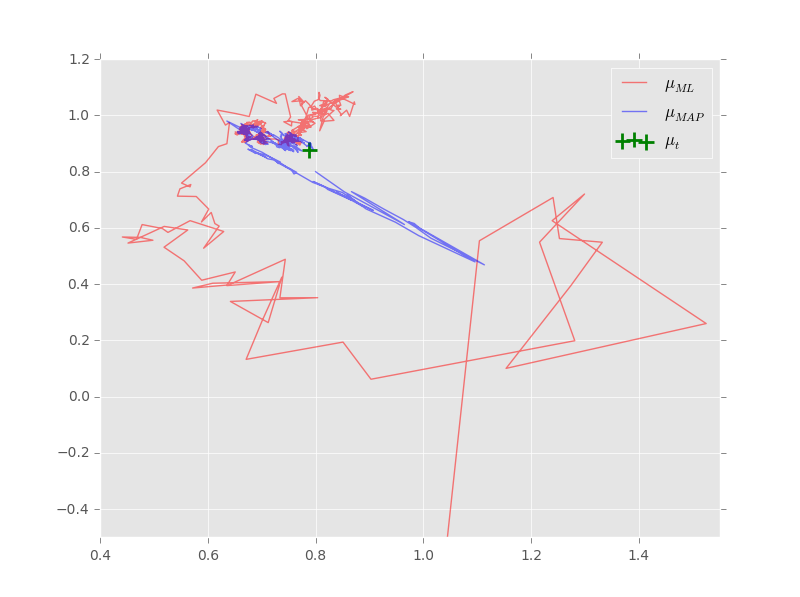
\includegraphics[width=\linewidth]{trajectory.png}
	\caption{A contour plot with the gradient descent trajectory overlaid. The number of iterations surpasses 70000, which is due to the fact that only small steps can be taken. If the value for $\eta$ is too high, the algorithm will move out of the valley, which will only slow down convergence even more. Zooming in shows a zig zag pattern.}
\end{figure}

As shown in the figure, convergence is very slow. Over 70000 iterations are needed for convergence. This is due to the fact that the slope in the valley is so low. 

\section{Probability theory}
\subsection{Apples and grapefruits}

\begin{equation}
	P(F_1 = \verb|apple| \vert F_2 = \verb|grapefruit|) = \frac{4}{7} \cdot \frac{8}{12} + \frac{3}{7} \cdot \frac{15}{18} = \frac{31}{42} \approx 0.738
\end{equation}
The probability of the second pick can affect the probability of the first pick due to the fact that the two pieces of fruit are chosen from the same box. Knowing that the second pick is a grapefruit changes the probability of box 1 being chosen from $\frac{1}{2}$ to $\frac{4}{7}$.
\subsection{Oranges and grapefruits}
There are a total of five options:
\begin{itemize}
\item If you get an orange, you know it is from the first box, so the probability for picking a grapefruit next is $\frac{4}{24}$.
\item If you get a grapefruit, the probability for another grapefruit is $\frac{4}{7} \cdot \frac{4}{24} + \frac{3}{7} \cdot 3/18 = \frac{4}{24}$.
\item If you get an apple, the probability for a grapefruit is $\frac{8}{23} \cdot \frac{4}{24} + \frac{15}{23} \cdot 3/18 = \frac{4}{24}$.
\end{itemize}
This is all very logical since the probability for a grapefruit is the same in the two boxes: $\frac{4}{24}$ in box 1 and $\frac{3}{18} = \frac{4}{24}$ in box 2.

I would say the two picks are still dependent, it is just that the probabilities in the two boxes are equal for the grapefruits. If these probabilities were to change, the dependency would show again.
\end{document}